\documentclass{article}
\usepackage[a4paper]{geometry}
\usepackage[utf8]{inputenc}
\DeclareUnicodeCharacter{00A0}{ }
\usepackage[english, italian]{babel}
\usepackage{parskip}
\usepackage{etaremune}
\usepackage{appendix}
\renewcommand\appendixtocname{Appendici}
\setcounter{secnumdepth}{4}
\setcounter{tocdepth}{4}
\usepackage[usenames,dvipsnames]{color}
\usepackage{titlesec}
\usepackage{float}
\usepackage[colorlinks=true]{hyperref}
\hypersetup{
    colorlinks=true,
    citecolor=black,
    filecolor=black,
    linkcolor=black,
    urlcolor=blue
}
\usepackage{breakurl}
\usepackage{graphicx}
\usepackage{lastpage}
\usepackage{longtable}
\usepackage{booktabs}
\usepackage{tabularx}
\usepackage{multirow}
\usepackage{longtable}
\usepackage[table]{xcolor}
\usepackage{tabu}
\setlength{\tabulinesep}{6pt}
\usepackage{array}
\usepackage{ragged2e}
\newcolumntype{P}[1]{>{\RaggedRight\hspace{0pt}}p{#1}}
\usepackage{fancyhdr}
\usepackage{textcomp}
\usepackage{changepage}
\usepackage{pgfplots}
\usepackage{tikz}
\usepackage{grffile}
\usepackage{rotating}
\usepackage{calc}
\fancypagestyle{plain}{
	% cancella tutti i campi di intestazione e piè di pagina
	\fancyhf{}

	\lhead{
		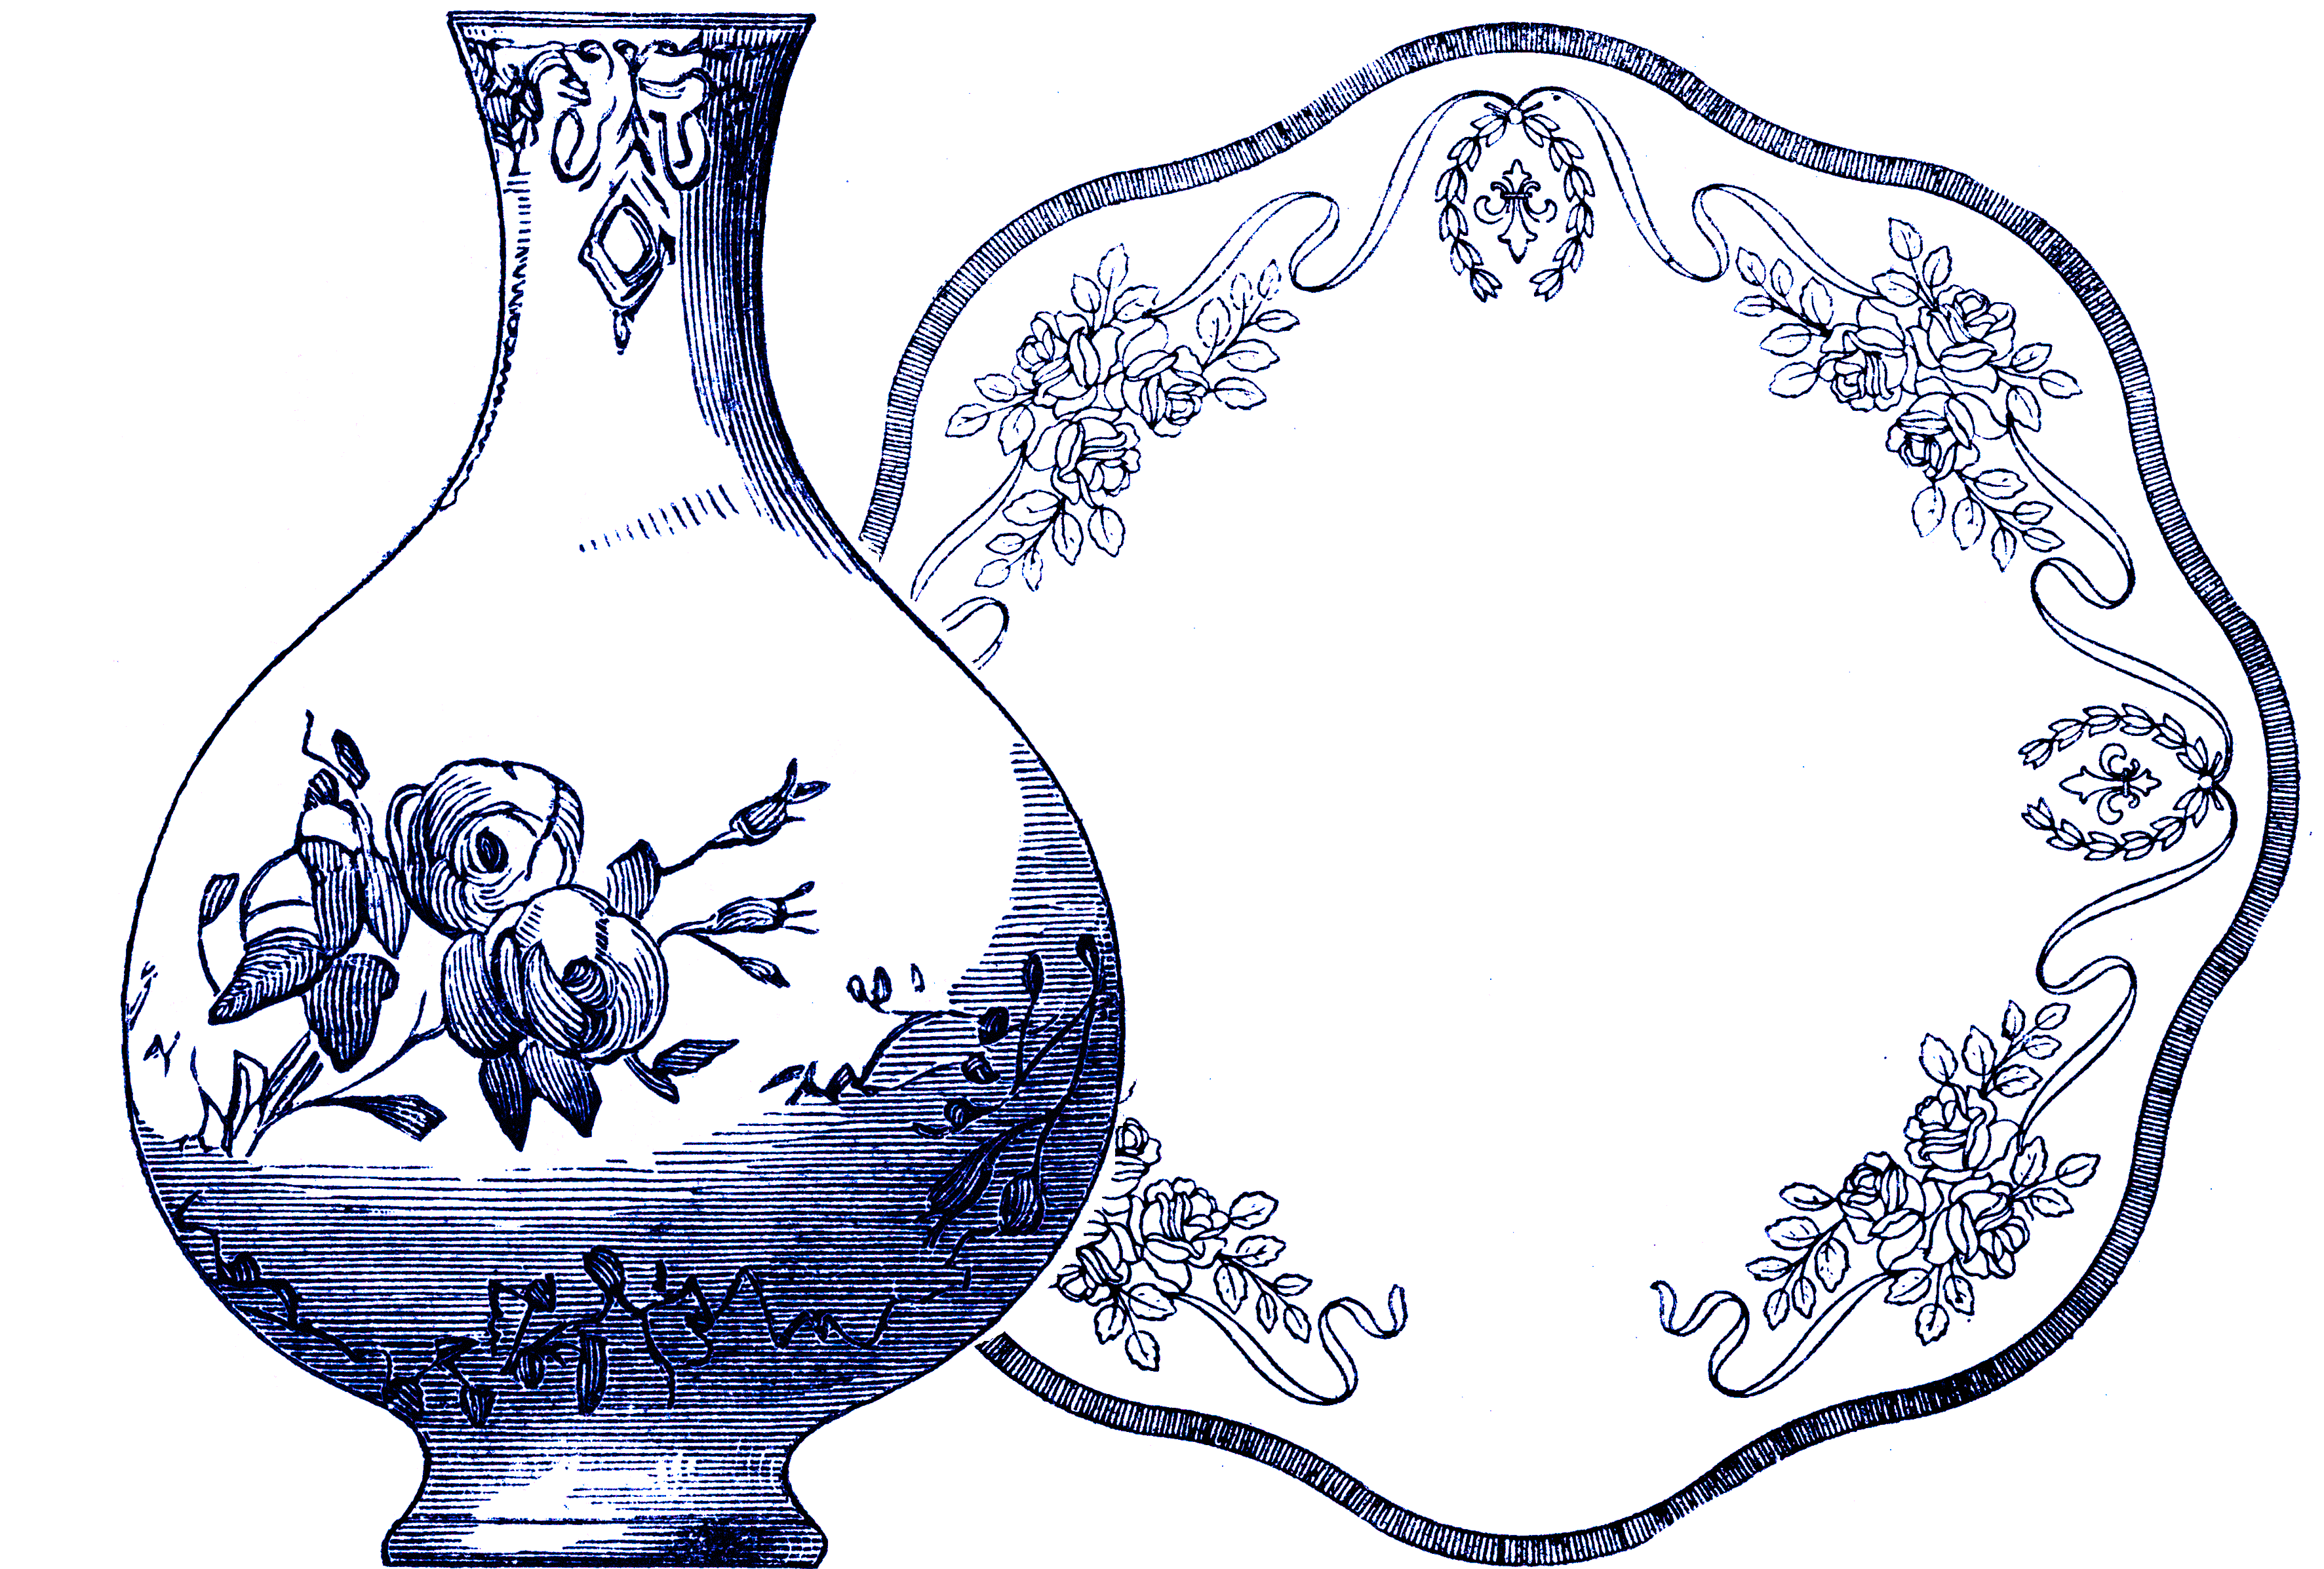
\includegraphics[height=1.5cm, width=1.5cm, keepaspectratio=true]{logo.png}
		\parbox[b]{10cm}{
			\emph{\ProjectName{}} \vspace{7pt}
		}
	}
	\chead{}
	\rhead{
		\slshape \leftmark
	}

	\lfoot{
		\ProjectName{}
	}
	\rfoot{Pagina \thepage{} di \pageref{LastPage}}
	\renewcommand{\headrulewidth}{0.3pt}
	\renewcommand{\footrulewidth}{0.3pt}
}
\setlength{\headheight}{30pt}
\pagestyle{plain}
\usepackage{listings}
\lstset{
  extendedchars=true,          % lets you use non-ASCII characters
  inputencoding=utf8,   % converte i caratteri utf8 in latin1, richiede \usepackage{listingsutf8} anzichè listings
  basicstyle=\ttfamily,        % the size of the fonts that are used for the code
  breakatwhitespace=false,     % sets if automatic breaks should only happen at whitespace
  breaklines=true,             % sets automatic line breaking
  captionpos=t,                % sets the caption-position to top
  commentstyle=\color{mygreen},   % comment style
  frame=none,               % adds a frame around the code
  keepspaces=true,            % keeps spaces in text, useful for keeping indentation of code (possibly needs columns=flexible)
  keywordstyle=\bfseries,     % keyword style
  numbers=none,               % where to put the line-numbers; possible values are (none, left, right)
  numbersep=5pt,              % how far the line-numbers are from the code
  numberstyle=\color{mygray}, % the style that is used for the line-numbers
  rulecolor=\color{black},    % if not set, the frame-color may be changed on line-breaks within not-black text (e.g. comments (green here))
  showspaces=false,           % show spaces everywhere adding particular underscores; it overrides 'showstringspaces'
  showstringspaces=false,     % underline spaces within strings only
  showtabs=false,             % show tabs within strings adding particular underscores
  stepnumber=5,               % the step between two line-numbers. If it's 1, each line will be numbered
  stringstyle=\color{red},    % string literal style
  tabsize=4,                  % sets default tabsize
  firstnumber=1      % visualizza i numeri dalla prima linea
}
\usepackage[T1]{fontenc}
\usepackage{lmodern}